\documentclass{beamer}
\usefonttheme[onlymath]{serif}
\usepackage{amsmath}
\usepackage{amsfonts}
\usepackage[export]{adjustbox}
\usepackage[utf8]{inputenc}
\usepackage{tikz} 
\usetikzlibrary{bayesnet}

% definitions
\def\H{\mathcal{H}}
\def\X{\mathbf{X}}
\def\w{\mathbf{w}}
\def\W{\mathbf{W}}
\def\const{\mathrm{const}}
\def\Var{\mathrm{Var}}
\def\tr{\mathrm{tr}}
\def\T{\top}
\def\U{\mathbf{U}}
\def\S{\mathbf{S}}
\def\V{\mathbf{V}}
\def\N{\mathcal{N}}
\def\E{\mathbb{E}}
\newcommand{\argmin}{\mathop{\mathrm{argmin}}}
\newcommand{\argmax}{\mathop{\mathrm{argmax}}}
\newcommand{\minimize}{\mathop{\mathrm{minimize}}}
\newcommand{\maximize}{\mathop{\mathrm{maximize}}}
\newcommand{\st}{\mathop{\mathrm{subject\,\,to}}}

%Information to be included in the title page:
\usecolortheme{seahorse}
\title{Infomation Criterion}
\author{Thomas Bayes}
\institute{
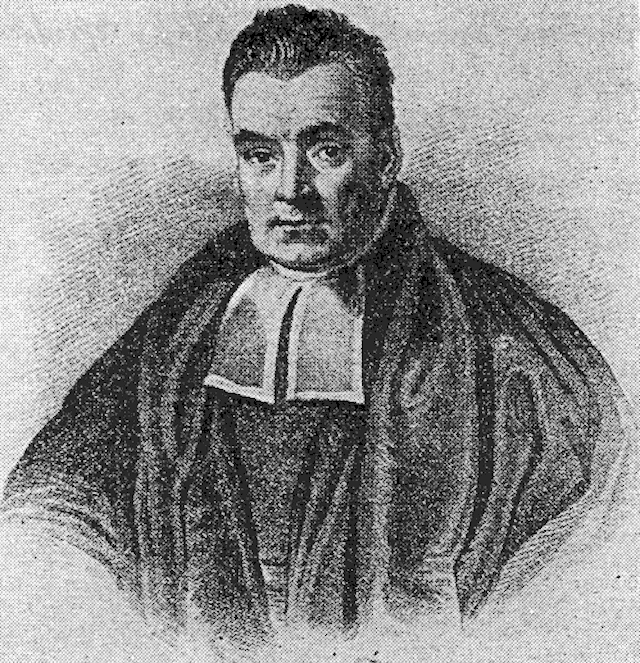
\includegraphics[height=.3\textheight]{../bayes.png}%
}
\date{\today}

    
    
\begin{document}
    
\frame{\titlepage}

\begin{frame}{Introduction}
In this slides, we are going to introduce the following concept.
\begin{itemize}
\item Laplace approximation
\item BIC
\item AIC
\end{itemize}
\end{frame}
\begin{frame}[allowframebreaks]{Laplace Approximation}
The idea of Laplace Approximation is use a Gaussian distribution to approximate a distribution.
$$p(z) = \frac{f(z)}{\int_z f(z) dz}$$
First we find the mode $z_0$ of the distribution
$$\frac{d f(z)}{dz} \Bigr|_{z=z_0} = 0$$
Then we evaluate the Hessian matrix $A$ at $z=z_0$, 
$$A = -\nabla^2 \ln f(z) \Bigr|_{z=z_0}$$
Then we approximate the function as 
$$\ln f(z) \approx \ln f(z_0) - \frac{1}{2} (z - z_0)^\top A (z - z_0)$$

\framebreak

Remark of Laplace's approximation
\end{frame}

\begin{frame}{BIC}
In context of model comparison, we are given a data set $\mathcal{D}$, and a set of models $\mathcal{M}_i$
We are interested in computing the model evidence, 
$$p(\mathcal{D} | \mathcal{M}_i) = \int p(\mathcal{D} | \theta, \mathcal{M}_i) p(\theta | \mathcal{M}_i) d\theta$$
Use 

\end{frame}




\end{document}